\documentclass[11pt]{article}

\usepackage{graphicx}
\usepackage{amsmath,amsthm,amssymb,color,latexsym}
\usepackage{enumitem,cancel}
\usepackage{listings}
\usepackage{xcolor}
\usepackage{hyperref}
\usepackage{tabularray}

\tolerance 99999
\hbadness 99999

\definecolor{codegreen}{rgb}{0,0.6,0}
\definecolor{codegray}{rgb}{0.5,0.5,0.5}
\definecolor{codepurple}{rgb}{0.58,0,0.82}
\definecolor{backcolour}{rgb}{0.99,0.99,0.97}

\lstdefinestyle{mystyle}{
    backgroundcolor=\color{backcolour},
    commentstyle=\color{codegreen},
    keywordstyle=\color{magenta},
    numberstyle=\tiny\color{codegray},
    stringstyle=\color{codepurple},
    basicstyle=\ttfamily\footnotesize,
    breakatwhitespace=false,
    breaklines=true,
    captionpos=b,
    keepspaces=true,
    numbers=left,
    numbersep=5pt,
    showspaces=false,
    showstringspaces=false,
    showtabs=false,
    tabsize=2
}

\lstset{style=mystyle}


% Margins
\topmargin=-0.45in
\evensidemargin=0in
\oddsidemargin=0in
\textwidth=6.5in
\textheight=9.0in
\headsep=0.25in

\newenvironment{points}{\vspace{0.3cm} \begin{enumerate}[label={(\alph*)}]}{\end{enumerate} \vspace{0.2cm}}


\title{ Design and Analysis of Software Systems \\ Assignment - 3 \\ IMS Design}
\author{ Abhiram Tilak - 2022113011 \\ Moida Praneeth Jain - 2022101093 }
\date{\today}

\begin{document}
\maketitle

\section{Software Used}

We have used StarUML to design the class and state diagrams,
and \LaTeX  for the report.

The figure \ref{class} is a high resolution image of the class diagram. In case the image is blurry, 
use the following drive link to get access to the files in pdf, jpeg and staruml (mdj) formats.

\textbf{Drive Link}: TODO


\section{Class Diagram}

\pagebreak

\begin{figure}[!ht]
    \center
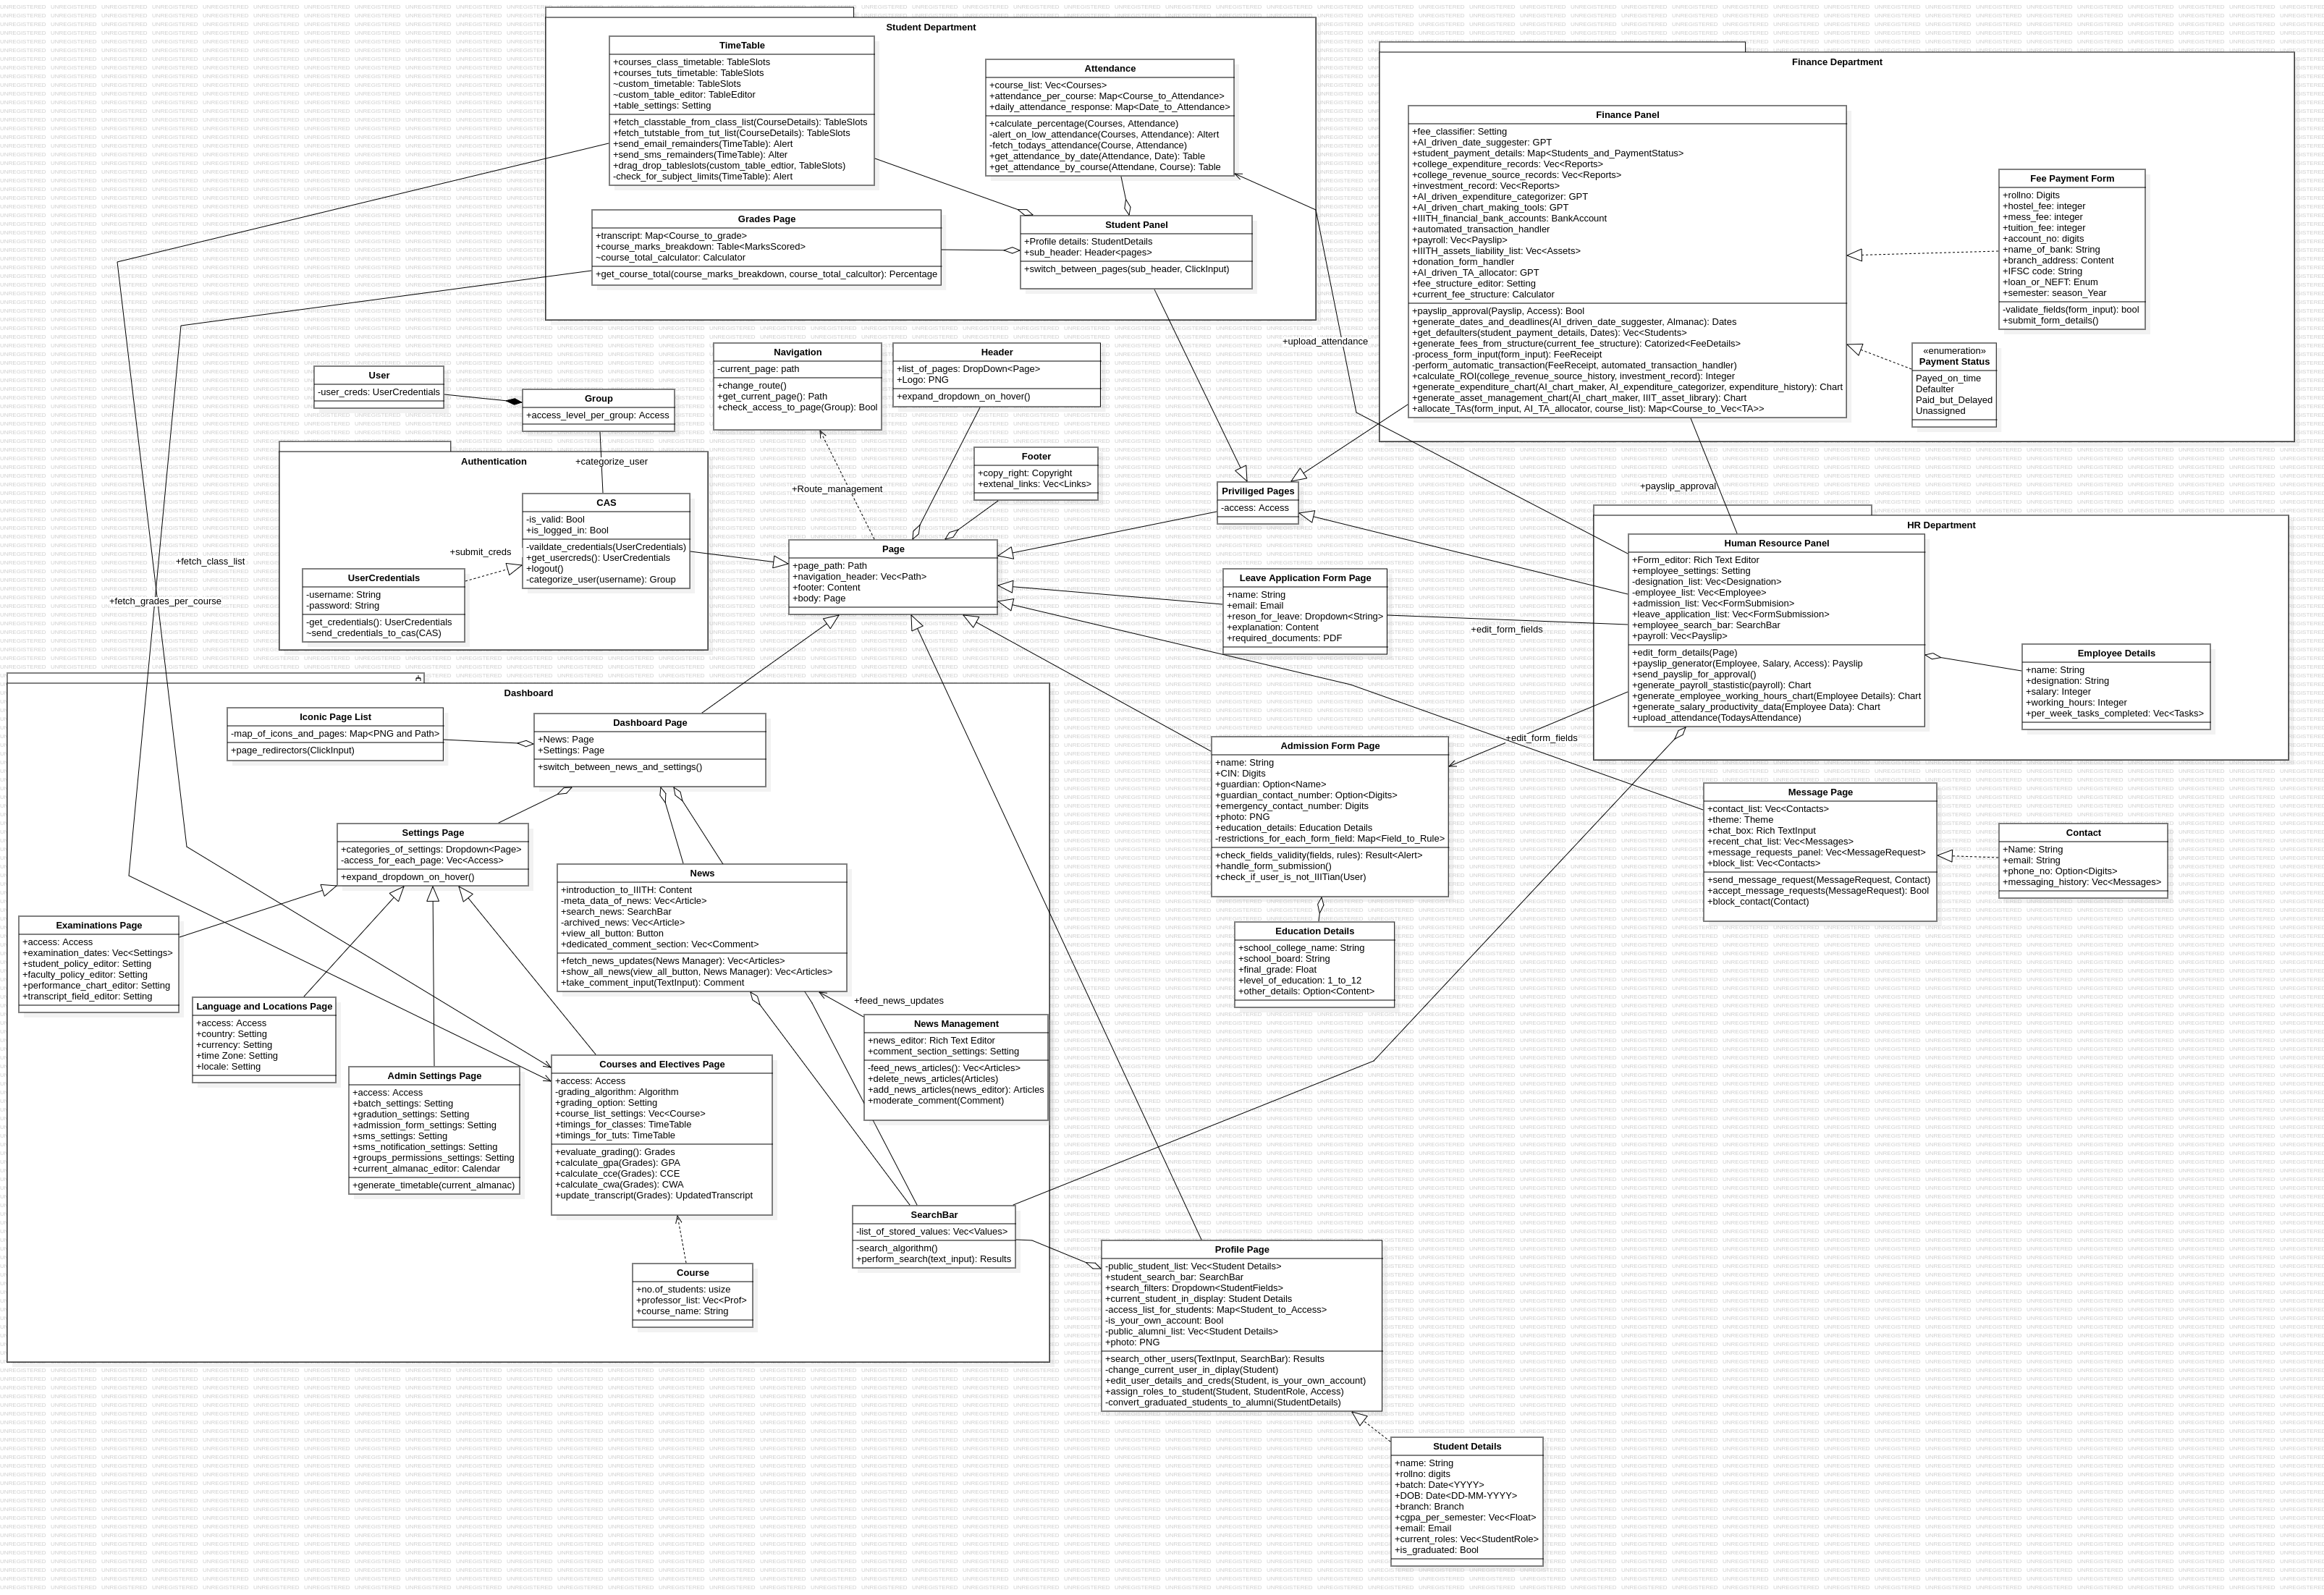
\includegraphics[width=8in,angle=90]{class_diagram/Main.png}
\caption{Class Diagram for IMS}
\label{class}
\end{figure}

\pagebreak

\begin{longtblr}[
  label = none,
  entry = none,
]{
  cell{1}{1} = {r=2}{},
  vlines,
  hline{1,3} = {-}{},
  hline{2} = {2}{},
}
User & {\textbf{Class State: }Is a basic unit of a user of IMS, containing a unique\\ username(email)
and password.\\\labelitemi\hspace{\dimexpr\labelsep+0.5\tabcolsep}User Credentials} \\
     &
\end{longtblr}

\begin{longtblr}[
  label = none,
  entry = none,
]{
  cell{1}{1} = {r=2}{},
  vlines,
  hline{1,3} = {-}{},
  hline{2} = {2}{},
}
Group & {\textbf{Class State: }Group is a basic categorization of Users to \\
have special access and privileges\\\labelitemi\hspace{\dimexpr\labelsep+0.5\tabcolsep}Access Level} \\
      &
\end{longtblr}

\begin{longtblr}[
  label = none,
  entry = none,
]{
  cell{1}{1} = {r=2}{},
  vlines,
  hline{1,3} = {-}{},
  hline{2} = {2}{},
}
UserCredentials & {\textbf{Class State: }Contents of form input after the person enters details.\\
\labelitemi\hspace{\dimexpr\labelsep+0.5\tabcolsep}Is\_Valid\_User\\
\labelitemi\hspace{\dimexpr\labelsep+0.5\tabcolsep}Is\_Logged\_In}\\
                & {\labelitemi\hspace{\dimexpr\labelsep+0.5\tabcolsep}get\_credentials(): Takes form input and
converts it into \\credentials to be passed to CAS.\\
\labelitemi\hspace{\dimexpr\labelsep+0.5\tabcolsep}send\_credentials\_to\_cas(): Sends credentials to external CAS\\
in json format.}
\end{longtblr}


\begin{longtblr}[
  label = none,
  entry = none,
]{
  cell{1}{1} = {r=2}{},
  vlines,
  hline{1,3} = {-}{},
  hline{2} = {2}{},
}
CAS & {\textbf{Class State: }Central Authentication system, used to validate IIIT\\credentials.\\\labelitemi\hspace{\dimexpr\labelsep+0.5\tabcolsep}Is\_Valid\_User\\\labelitemi\hspace{\dimexpr\labelsep+0.5\tabcolsep}Is\_Logged\_In}                                                                                                                                                                \\
    & {\labelitemi\hspace{\dimexpr\labelsep+0.5\tabcolsep}Validate User Credentials(): Used to validate
user credentials given as input\\
\labelitemi\hspace{\dimexpr\labelsep+0.5\tabcolsep}Get User Credentials(): Used
to get the from from the submission page.\\
\labelitemi\hspace{\dimexpr\labelsep+0.5\tabcolsep}Categorize User(): After authentication tries to classify user \\
and give sufficient Access.}
\end{longtblr}

\begin{longtblr}[
  label = none,
  entry = none,
]{
  cell{1}{1} = {r=2}{},
  vlines,
  hline{1,3} = {-}{},
  hline{2} = {2}{},
}
Page & {\textbf{Class State: }Contains basic skeleton of each page of the website or the portal\\
\labelitemi\hspace{\dimexpr\labelsep+0.5\tabcolsep}Page Path\\
\labelitemi\hspace{\dimexpr\labelsep+0.5\tabcolsep}Navigation Header\\
\labelitemi\hspace{\dimexpr\labelsep+0.5\tabcolsep}Footer\\
\labelitemi\hspace{\dimexpr\labelsep+0.5\tabcolsep}Body} \\
     &
\end{longtblr}

\begin{longtblr}[
  label = none,
  entry = none,
]{
  cell{1}{1} = {r=2}{},
  vlines,
  hline{1,3} = {-}{},
  hline{2} = {2}{},
}
Footer & {\textbf{Class State: }Footer located at the bottom of the webpage\\
\labelitemi\hspace{\dimexpr\labelsep+0.5\tabcolsep}Copyright\\
\labelitemi\hspace{\dimexpr\labelsep+0.5\tabcolsep}External Links} \\
       &
\end{longtblr}


% \usepackage{tabularray}
\begin{longtblr}[
  label = none,
  entry = none,
]{
  cell{1}{1} = {r=2}{},
  vlines,
  hline{1,3} = {-}{},
  hline{2} = {2}{},
}
Header & {\textbf{Class State: }Header at the top of the page used for navigation\\
\labelitemi\hspace{\dimexpr\labelsep+0.5\tabcolsep}Dropdown of pages\\
\labelitemi\hspace{\dimexpr\labelsep+0.5\tabcolsep}IIIT Logo} \\
       &
\end{longtblr}


\begin{longtblr}[
  label = none,
  entry = none,
]{
  cell{1}{1} = {r=2}{},
  vlines,
  hline{1,3} = {-}{},
  hline{2} = {2}{},
}
Navigation & {\textbf{Class State: }Handles backend navigation and routing between pages visited\\
\labelitemi\hspace{\dimexpr\labelsep+0.5\tabcolsep}Current Page}\\
           & {\textbf{Class Behavior}\\
\labelitemi\hspace{\dimexpr\labelsep+0.5\tabcolsep}change\_route(): Used to handle changing
the path of the page and \\ redirect to the next one\\
\labelitemi\hspace{\dimexpr\labelsep+0.5\tabcolsep}get\_current\_page(): Get the path of the current
page, used for \\ displaying and redirection\\
\labelitemi\hspace{\dimexpr\labelsep+0.5\tabcolsep}check\_access\_to\_page(): Get the access levels of
each page and \\ show a trespassing alert otherwise}
\end{longtblr}

% \usepackage{tabularray}
\begin{longtblr}[
  label = none,
  entry = none,
]{
  cell{1}{1} = {r=2}{},
  vlines,
  hline{1,3} = {-}{},
  hline{2} = {2}{},
}
Dashboard & {\textbf{Class State: }The main and the opening page of the portal which has \\most features
common but some items can be not displayed or displayed \\based on Access.\\
\labelitemi\hspace{\dimexpr\labelsep+0.5\tabcolsep}News\\
\labelitemi\hspace{\dimexpr\labelsep+0.5\tabcolsep}Page} \\
          & {\textbf{Class Behavior}\\\labelitemi\hspace{\dimexpr\labelsep+0.5\tabcolsep}switch\_between\_news\_and\_settings():
By default only one of News or\\ settings page is shown to view.}
\end{longtblr}

\begin{longtblr}[
  label = none,
  entry = none,
]{
  cell{1}{1} = {r=2}{},
  vlines,
  hline{1,3} = {-}{},
  hline{2} = {2}{},
}
SearchBar & {\textbf{Class State: } Template search bar.\\
\labelitemi\hspace{\dimexpr\labelsep+0.5\tabcolsep}List of stored values} \\
          & {\textbf{Class Behavior}\\\labelitemi\hspace{\dimexpr\labelsep+0.5\tabcolsep}search\_algorithm():
This defines the algorithm used to prioritize search results, \\
leniency in matching results, etc.\\
\labelitemi\hspace{\dimexpr\labelsep+0.5\tabcolsep}perform\_search(): Handles search when text input
 is \\specified and displays results.}
\end{longtblr}


\begin{longtblr}[
  label = none,
  entry = none,
]{
  cell{1}{1} = {r=2}{},
  vlines,
  hline{1,3} = {-}{},
  hline{2} = {2}{},
}
Page List & {\textbf{Class State: }List of clickable icons used for\\ user friendly navigation.\\
\labelitemi\hspace{\dimexpr\labelsep+0.5\tabcolsep}Map of icons and page} \\
                 & {\textbf{Class Behavior}\\\labelitemi\hspace{\dimexpr\labelsep+0.5\tabcolsep}page\_re-directors():
Used to handle redirection to respective pages when \\icons are clicked on}
\end{longtblr}


\begin{longtblr}[
  label = none,
  entry = none,
]{
  cell{1}{1} = {r=2}{},
  vlines,
  hline{1,3} = {-}{},
  hline{2} = {2}{},
}
Settings Page & {\textbf{Class State: }Sample Settings page containing different types of settings
with \\different level of access\\
\labelitemi\hspace{\dimexpr\labelsep+0.5\tabcolsep}Categories of settings\\
\labelitemi\hspace{\dimexpr\labelsep+0.5\tabcolsep}Access for each Page} \\
              & {\textbf{Class Behavior}\\
\labelitemi\hspace{\dimexpr\labelsep+0.5\tabcolsep}expand\_dropdown\_on\_hover(): Each settings
page contains various settings \\which will be divided into various categories.}
\end{longtblr}

\begin{longtblr}[
  label = none,
  entry = none,
]{
  cell{1}{1} = {r=2}{},
  vlines,
  hline{1,3} = {-}{},
  hline{2} = {2}{},
}
Examination Page & {\textbf{Class State: }Page used by Exam Cell for changing settings related \\
examination, dates, policies etc.\\
\labelitemi\hspace{\dimexpr\labelsep+0.5\tabcolsep}Access\\
\labelitemi\hspace{\dimexpr\labelsep+0.5\tabcolsep}Examination Dates\\
\labelitemi\hspace{\dimexpr\labelsep+0.5\tabcolsep}Student Policy Editor\\
\labelitemi\hspace{\dimexpr\labelsep+0.5\tabcolsep}Faculty Policy Editor\\
\labelitemi\hspace{\dimexpr\labelsep+0.5\tabcolsep}Performance Chart Editor\\
\labelitemi\hspace{\dimexpr\labelsep+0.5\tabcolsep}Transcript field editor} \\
                 &
\end{longtblr}


% \usepackage{tabularray}
\begin{longtblr}[
  label = none,
  entry = none,
]{
  cell{1}{1} = {r=2}{},
  vlines,
  hline{1,3} = {-}{},
  hline{2} = {2}{},
}
Language and Locations & {\textbf{Class State: }Page with settings related to language and location
\\settings, accessible to all users.\\
\labelitemi\hspace{\dimexpr\labelsep+0.5\tabcolsep}Access\\
\labelitemi\hspace{\dimexpr\labelsep+0.5\tabcolsep}Country\\
\labelitemi\hspace{\dimexpr\labelsep+0.5\tabcolsep}Currency\\
\labelitemi\hspace{\dimexpr\labelsep+0.5\tabcolsep}Time Zones\\
\labelitemi\hspace{\dimexpr\labelsep+0.5\tabcolsep}Locale} \\
                       &
\end{longtblr}


\begin{longtblr}[
  label = none,
  entry = none,
]{
  cell{1}{1} = {r=2}{},
  vlines,
  hline{1,3} = {-}{},
  hline{2} = {2}{},
}
Admin Settings Page & {\textbf{Class State: }Contains Administrator Settings related to the whole\\ IMS
portal like SMS settings. Also contains settings related to \\graduation and admission.\\
\labelitemi\hspace{\dimexpr\labelsep+0.5\tabcolsep}Access\\
\labelitemi\hspace{\dimexpr\labelsep+0.5\tabcolsep}Batch Settings\\
\labelitemi\hspace{\dimexpr\labelsep+0.5\tabcolsep}Graduation Settings\\
\labelitemi\hspace{\dimexpr\labelsep+0.5\tabcolsep}Admission Form Settings\\
\labelitemi\hspace{\dimexpr\labelsep+0.5\tabcolsep}SMS Settings\\
\labelitemi\hspace{\dimexpr\labelsep+0.5\tabcolsep}SMS Notification Settings\\
\labelitemi\hspace{\dimexpr\labelsep+0.5\tabcolsep}Group Permissions Settings\\
\labelitemi\hspace{\dimexpr\labelsep+0.5\tabcolsep}Almanac / Calendar Settings} \\
                    & {\textbf{Class Behavior}\\\labelitemi\hspace{\dimexpr\labelsep+0.5\tabcolsep}
Generate Time Table(): Handles generate time tables from \\the current Settings and configuration}
\end{longtblr}

\begin{longtblr}[
  label = none,
  entry = none,
]{
  cell{1}{1} = {r=2}{},
  vlines,
  hline{1,3} = {-}{},
  hline{2} = {2}{},
}
Course and Electives Page & {\textbf{Class State: }Settings page usually used by faculty to \\
change things like grading, and also set classes\\ and tutorials.\\
\labelitemi\hspace{\dimexpr\labelsep+0.5\tabcolsep}Access\\
\labelitemi\hspace{\dimexpr\labelsep+0.5\tabcolsep}Grading Algorithm\\
\labelitemi\hspace{\dimexpr\labelsep+0.5\tabcolsep}Grading Option\\
\labelitemi\hspace{\dimexpr\labelsep+0.5\tabcolsep}Course List Setting\\
\labelitemi\hspace{\dimexpr\labelsep+0.5\tabcolsep}Timings for Classes\\
\labelitemi\hspace{\dimexpr\labelsep+0.5\tabcolsep}Timings for Tutorials} \\
                          & {\textbf{Class Behavior}\\
\labelitemi\hspace{\dimexpr\labelsep+0.5\tabcolsep}evaluate\_grade(): Use the grading algorithm to find the grades.\\
\labelitemi\hspace{\dimexpr\labelsep+0.5\tabcolsep}calculate\_gpa(): Used to calculate GPA from grades\\
\labelitemi\hspace{\dimexpr\labelsep+0.5\tabcolsep}calculate\_cce(): Used to calculate CCE from grades\\
\labelitemi\hspace{\dimexpr\labelsep+0.5\tabcolsep}calculate\_cwa(): Used to calculate CWA from grades\\
\labelitemi\hspace{\dimexpr\labelsep+0.5\tabcolsep}update\_transcript(): Updates the transcript from the grades \\
calculated from each course.}
\end{longtblr}


\begin{longtblr}[
  label = none,
  entry = none,
]{
  cell{1}{1} = {r=2}{},
  vlines,
  hline{1,3} = {-}{},
  hline{2} = {2}{},
}
News & {\textbf{Class State: }This is the default body of the dashboard page. contains news articles \\
which has a separate management class to change the content. \\
\labelitemi\hspace{\dimexpr\labelsep+0.5\tabcolsep}Introduction to IIITH \\
\labelitemi\hspace{\dimexpr\labelsep+0.5\tabcolsep}Meta Data of News\\
\labelitemi\hspace{\dimexpr\labelsep+0.5\tabcolsep}Search News\\
\labelitemi\hspace{\dimexpr\labelsep+0.5\tabcolsep}Archived News\\
\labelitemi\hspace{\dimexpr\labelsep+0.5\tabcolsep}"View all" button\\
\labelitemi\hspace{\dimexpr\labelsep+0.5\tabcolsep}Dedicated Comment Section} \\
     & {\textbf{Class Behavior}\\
\labelitemi\hspace{\dimexpr\labelsep+0.5\tabcolsep}fetch\_news\_updates(): Used to fetch news updates
from the editable news update \\management panel\\
\labelitemi\hspace{\dimexpr\labelsep+0.5\tabcolsep}show\_all\_news(): When the "View All" buttons is pressed,
it expands to show all \\news up for display\\
\labelitemi\hspace{\dimexpr\labelsep+0.5\tabcolsep}take\_comment\_input(): Handle posting comments in the comment
section if \\there is access.}
\end{longtblr}


\begin{longtblr}[
  label = none,
  entry = none,
]{
  cell{1}{1} = {r=2}{},
  vlines,
  hline{1,3} = {-}{},
  hline{2} = {2}{},
}
News Management & {\textbf{Class State: }Management component used for generating content and \\
moderating the comments of the News articles. This can be accessed by \\News
Moderators. \\
\labelitemi\hspace{\dimexpr\labelsep+0.5\tabcolsep}News Editor\\
\labelitemi\hspace{\dimexpr\labelsep+0.5\tabcolsep}Comment Section Settings}\\
                & {\textbf{Class Behavior}\\
\labelitemi\hspace{\dimexpr\labelsep+0.5\tabcolsep}feed\_news\_articles(): Used to feed the dashboard page with latest\\ news
whenever fetched for updates.\\
\labelitemi\hspace{\dimexpr\labelsep+0.5\tabcolsep}delete\_news\_articles(): Used to delete older news articles\\
\labelitemi\hspace{\dimexpr\labelsep+0.5\tabcolsep}add\_news\_articles(): Used
to add new articles from the Rich text \\editor \\
\labelitemi\hspace{\dimexpr\labelsep+0.5\tabcolsep}moderate\_comments(): Use the delete, flag, report comments by \\
administrator.}
\end{longtblr}


\begin{longtblr}[
  label = none,
  entry = none,
]{
  cell{1}{1} = {r=2}{},
  vlines,
  hline{1,3} = {-}{},
  hline{2} = {2}{},
}
Profile Page & {\textbf{Class State: }Page visible to every user dedicated to showing user details and \\
also supports finding other users, students, alumni and find their level of access \\to IMS. \\
\labelitemi\hspace{\dimexpr\labelsep+0.5\tabcolsep}Public Student List\\
\labelitemi\hspace{\dimexpr\labelsep+0.5\tabcolsep}Student Search Bar\\
\labelitemi\hspace{\dimexpr\labelsep+0.5\tabcolsep}Search Filters\\
\labelitemi\hspace{\dimexpr\labelsep+0.5\tabcolsep}Current Student in Display\\
\labelitemi\hspace{\dimexpr\labelsep+0.5\tabcolsep}Access List for students\\
\labelitemi\hspace{\dimexpr\labelsep+0.5\tabcolsep}is\_your\_account\\
\labelitemi\hspace{\dimexpr\labelsep+0.5\tabcolsep}Public Alumni List} \\
             & {\textbf{Class Behavior}\\
\labelitemi\hspace{\dimexpr\labelsep+0.5\tabcolsep}search\_other\_students(): Use the search bar to search
other students and \\ alumni and display the results\\
\labelitemi\hspace{\dimexpr\labelsep+0.5\tabcolsep}change\_current\_user\_in\_display(): Used to handle the
current user details \\that are shown in the placeholder.\\
\labelitemi\hspace{\dimexpr\labelsep+0.5\tabcolsep}edit\_user\_details\_and\_creds(): Gives the
ability to edit some of the profile \\details depending on if the signed-in user is trying to edit his own account.\\
\labelitemi\hspace{\dimexpr\labelsep+0.5\tabcolsep}assign\_roles\_to\_students(): Users with enough privileges can
assign roles to \\users. This roles have no purpose in IMS and are different groups.\\
\labelitemi\hspace{\dimexpr\labelsep+0.5\tabcolsep}convert\_graduated\_students\_to\_alumni(): Automated function that\\
converts graduated students to alumni}
\end{longtblr}

\begin{longtblr}[
  label = none,
  entry = none,
]{
  cell{1}{1} = {r=2}{},
  vlines,
  hline{1,3} = {-}{},
  hline{2} = {2}{},
}
Student Details & {\textbf{Class State: }This is a structure containing all student details at the\\ present State.\\
\labelitemi\hspace{\dimexpr\labelsep+0.5\tabcolsep}Name\\
\labelitemi\hspace{\dimexpr\labelsep+0.5\tabcolsep}Roll No\\
\labelitemi\hspace{\dimexpr\labelsep+0.5\tabcolsep}Batch\\
\labelitemi\hspace{\dimexpr\labelsep+0.5\tabcolsep}Date of Birth\\
\labelitemi\hspace{\dimexpr\labelsep+0.5\tabcolsep}Branch\\
\labelitemi\hspace{\dimexpr\labelsep+0.5\tabcolsep}CGPA\\
\labelitemi\hspace{\dimexpr\labelsep+0.5\tabcolsep}email\\
\labelitemi\hspace{\dimexpr\labelsep+0.5\tabcolsep}current\_roles\\
\labelitemi\hspace{\dimexpr\labelsep+0.5\tabcolsep}is\_graduated} \\
                &
\end{longtblr}


\begin{longtblr}[
  label = none,
  entry = none,
]{
  cell{1}{1} = {r=2}{},
  vlines,
  hline{1,3} = {-}{},
  hline{2} = {2}{},
}
Admission Form Page & {\textbf{Class State:} Admission form which is available if the user is not \\
recognized as a IIITian\\
\labelitemi\hspace{\dimexpr\labelsep+0.5\tabcolsep}Name\\
\labelitemi\hspace{\dimexpr\labelsep+0.5\tabcolsep}CIN\\
\labelitemi\hspace{\dimexpr\labelsep+0.5\tabcolsep}Guardian Name\\
\labelitemi\hspace{\dimexpr\labelsep+0.5\tabcolsep}Guardian Contact Number\\
\labelitemi\hspace{\dimexpr\labelsep+0.5\tabcolsep}Emergency Contact Number\\
\labelitemi\hspace{\dimexpr\labelsep+0.5\tabcolsep}Photo\\
\labelitemi\hspace{\dimexpr\labelsep+0.5\tabcolsep}Education Details\\
\labelitemi\hspace{\dimexpr\labelsep+0.5\tabcolsep}Restrictions for each form field} \\
                    & {\textbf{Class Behavior:}\\
\labelitemi\hspace{\dimexpr\labelsep+0.5\tabcolsep}check\_fields\_validity(): Checks if all fields are entered properly\\
 with constraints\\
\labelitemi\hspace{\dimexpr\labelsep+0.5\tabcolsep}handle\_form\_submissions(): Record all the form details and convert\\
 into JSON format\\
\labelitemi\hspace{\dimexpr\labelsep+0.5\tabcolsep}check\_if\_user\_is\_not\_IIITian(): This check is to control page\\
 visibility}
\end{longtblr}

\pagebreak

\begin{longtblr}[
  label = none,
  entry = none,
]{
  cell{1}{1} = {r=2}{},
  vlines,
  hline{1,3} = {-}{},
  hline{2} = {2}{},
}
Human Resource Panel & {\textbf{Class State:} Privileged page for Human Resource Employees used\\ to perform various actions.\\
\labelitemi\hspace{\dimexpr\labelsep+0.5\tabcolsep}Admission form editor\\
\labelitemi\hspace{\dimexpr\labelsep+0.5\tabcolsep}Employee Settings\\
\labelitemi\hspace{\dimexpr\labelsep+0.5\tabcolsep}Designation List\\
\labelitemi\hspace{\dimexpr\labelsep+0.5\tabcolsep}Employee List\\
\labelitemi\hspace{\dimexpr\labelsep+0.5\tabcolsep}Admission List\\
\labelitemi\hspace{\dimexpr\labelsep+0.5\tabcolsep}Leave Application List\\
\labelitemi\hspace{\dimexpr\labelsep+0.5\tabcolsep}Employee Search Bar\\
\labelitemi\hspace{\dimexpr\labelsep+0.5\tabcolsep}Payroll}\\
                     & {\textbf{Class Behavior:}\\
\labelitemi\hspace{\dimexpr\labelsep+0.5\tabcolsep}edit\_form\_details(): Used to edit forms like Leave application,
\\ Admission form.\\
\labelitemi\hspace{\dimexpr\labelsep+0.5\tabcolsep}payslip\_generator(): Have the ability to examine employee details\\
 and generate a payslip.\\
\labelitemi\hspace{\dimexpr\labelsep+0.5\tabcolsep}send\_payslip\_for\_approval(): Send payslip for approval to the
\\finance department\\
\labelitemi\hspace{\dimexpr\labelsep+0.5\tabcolsep}generate\_payroll\_statistics(): Use payroll data to generate a chart\\
\labelitemi\hspace{\dimexpr\labelsep+0.5\tabcolsep}generate\_employee\_working\_hour\_chart(): Take in data about
\\ employees and their working hours, and generate performance\\ charts.\\
\labelitemi\hspace{\dimexpr\labelsep+0.5\tabcolsep}generate\_salary\_productivity\_data(): Use the tasks completed
\\by employees and performance data to get the per capita\\ productivity chart.\\
\labelitemi\hspace{\dimexpr\labelsep+0.5\tabcolsep}Upload attendance: Upload the recorded attendance for the day\\
 and upload it. Shows up in the attendance page.}
\end{longtblr}


\begin{longtblr}[
  label = none,
  entry = none,
]{
  cell{1}{1} = {r=2}{},
  vlines,
  hline{1,3} = {-}{},
  hline{2} = {2}{},
}
Message Page & {\textbf{Class State:} A page dedicated to have messaging services among \\users of IMS\\
\labelitemi\hspace{\dimexpr\labelsep+0.5\tabcolsep}Contact List\\
\labelitemi\hspace{\dimexpr\labelsep+0.5\tabcolsep}Theme\\
\labelitemi\hspace{\dimexpr\labelsep+0.5\tabcolsep}Chat Box\\
\labelitemi\hspace{\dimexpr\labelsep+0.5\tabcolsep}Recent Chat List\\
\labelitemi\hspace{\dimexpr\labelsep+0.5\tabcolsep}Message Requests Panel\\
\labelitemi\hspace{\dimexpr\labelsep+0.5\tabcolsep}Block List}\\
             & {\textbf{Class Behavior:}\\
\labelitemi\hspace{\dimexpr\labelsep+0.5\tabcolsep}send\_message\_request(): Used to send a curated request to \\
the other IMS user contact, asking permissions to send messages\\
\labelitemi\hspace{\dimexpr\labelsep+0.5\tabcolsep}accept\_message\_requests: Used to accept message\\
 requests from a contact\\
\labelitemi\hspace{\dimexpr\labelsep+0.5\tabcolsep}block\_contact(): Used to block a contact and send
\\ it to Block list, messages from this user will not be displayed.}
\end{longtblr}

\begin{longtblr}[
  label = none,
  entry = none,
]{
  cell{1}{1} = {r=2}{},
  vlines,
  hline{1,3} = {-}{},
  hline{2} = {2}{},
}
Contact & {\textbf{Class State:} This is an abstraction of a user of IMS, contains information \\
that other user can see\\
\labelitemi\hspace{\dimexpr\labelsep+0.5\tabcolsep}Name\\
\labelitemi\hspace{\dimexpr\labelsep+0.5\tabcolsep}Email\\
\labelitemi\hspace{\dimexpr\labelsep+0.5\tabcolsep}Phone No\\
\labelitemi\hspace{\dimexpr\labelsep+0.5\tabcolsep}Messaging History} \\
        &
\end{longtblr}


\begin{longtblr}[
  label = none,
  entry = none,
]{
  cell{1}{1} = {r=2}{},
  vlines,
  hline{1,3} = {-}{},
  hline{2} = {2}{},
}
Fee Payment Form & {\textbf{Class State:} This is the form that students fill to perform \\online fee payment through IMS.\\
\labelitemi\hspace{\dimexpr\labelsep+0.5\tabcolsep}Roll No\\
\labelitemi\hspace{\dimexpr\labelsep+0.5\tabcolsep}Hostel Fees\\
\labelitemi\hspace{\dimexpr\labelsep+0.5\tabcolsep}Mess Fees\\
\labelitemi\hspace{\dimexpr\labelsep+0.5\tabcolsep}Tuition Fees\\
\labelitemi\hspace{\dimexpr\labelsep+0.5\tabcolsep}Account No\\
\labelitemi\hspace{\dimexpr\labelsep+0.5\tabcolsep}Name of the Bank\\
\labelitemi\hspace{\dimexpr\labelsep+0.5\tabcolsep}Branch Address\\
\labelitemi\hspace{\dimexpr\labelsep+0.5\tabcolsep}IFSC Code\\
\labelitemi\hspace{\dimexpr\labelsep+0.5\tabcolsep}{[}Loan or NEFT] ( Enum)\\
\labelitemi\hspace{\dimexpr\labelsep+0.5\tabcolsep}Semester} \\
                 & {\textbf{Class Behavior:}\\
\labelitemi\hspace{\dimexpr\labelsep+0.5\tabcolsep}validate\_fields(): Used to ensure if all the fields are filled \\
accordingly, and the form is valid\\
\labelitemi\hspace{\dimexpr\labelsep+0.5\tabcolsep}submit\_form\_details(): Used to submit form details, to be \\
process by finance department}
\end{longtblr}




\begin{longtblr}[
  label = none,
  entry = none,
]{
  cell{1}{1} = {r=2}{},
  vlines,
  hline{1,3} = {-}{},
  hline{2} = {2}{},
}
Finance Panel & {\textbf{Class State:} Privileged page for finance departments, contains tools \\
(AI driven), Settings, Databases, Form editors, \\Access to edit critical components like Fee Structure\\
\labelitemi\hspace{\dimexpr\labelsep+0.5\tabcolsep}Fee Classifier\\
\labelitemi\hspace{\dimexpr\labelsep+0.5\tabcolsep}AI Driven Date/Deadline
predictor\\
\labelitemi\hspace{\dimexpr\labelsep+0.5\tabcolsep}Student Payment Details\\
\labelitemi\hspace{\dimexpr\labelsep+0.5\tabcolsep}college expenditure records\\
\labelitemi\hspace{\dimexpr\labelsep+0.5\tabcolsep}college revenue source records\\
\labelitemi\hspace{\dimexpr\labelsep+0.5\tabcolsep}investment records\\
\labelitemi\hspace{\dimexpr\labelsep+0.5\tabcolsep}AI Driven Expenditure Classifier\\
\labelitemi\hspace{\dimexpr\labelsep+0.5\tabcolsep}AI Driven chart making tools\\
\labelitemi\hspace{\dimexpr\labelsep+0.5\tabcolsep}IIITH Financial bank accounts\\
\labelitemi\hspace{\dimexpr\labelsep+0.5\tabcolsep}automated transaction handler\\
\labelitemi\hspace{\dimexpr\labelsep+0.5\tabcolsep}payroll\\
\labelitemi\hspace{\dimexpr\labelsep+0.5\tabcolsep}IIITH asset liability list\\
\labelitemi\hspace{\dimexpr\labelsep+0.5\tabcolsep}donation form handler\\
\labelitemi\hspace{\dimexpr\labelsep+0.5\tabcolsep}fee structure editor\\
\labelitemi\hspace{\dimexpr\labelsep+0.5\tabcolsep}current fee strucutre}                                                                                                                                                                                                                                                                                 \\
              & {\textbf{Class Behavior:}\\
\labelitemi\hspace{\dimexpr\labelsep+0.5\tabcolsep}payslip\_approval(): Take payslip from HR team and approve it\\ after manual inspection.\\
\labelitemi\hspace{\dimexpr\labelsep+0.5\tabcolsep}generate\_dates\_and\_deadlines(): Use the AI \\
tools and manual intervention
\\to generate deadlines for fee submission and other financial processes.\\
\labelitemi\hspace{\dimexpr\labelsep+0.5\tabcolsep}get\_defaulters(): Use the deadline/dates info and the student
fee \\details to find out fee payment defaulters\\
\labelitemi\hspace{\dimexpr\labelsep+0.5\tabcolsep}generate\_fees\_from\_structure(): Use the current implementation of fee\\
 structure as input~ to calculate fees required to pay for each student\\
\labelitemi\hspace{\dimexpr\labelsep+0.5\tabcolsep}process\_form\_input(): Take the form input and make readable fields\\
 accepted by automatic transactor\\
\labelitemi\hspace{\dimexpr\labelsep+0.5\tabcolsep}perform\_automatic\_transaction(): Take fee information and perform \\
automatic online bank transfers\\
\labelitemi\hspace{\dimexpr\labelsep+0.5\tabcolsep}calculate\_roi(): Use the revenue, and investment and donations\\
 to calculate ROI of college\\
\labelitemi\hspace{\dimexpr\labelsep+0.5\tabcolsep}generate\_expenditure\_chart(): Use the expenditure records to\\
 generate a classification chart with detailed breakdown\\
\labelitemi\hspace{\dimexpr\labelsep+0.5\tabcolsep}generate\_asset\_management\_chart(): Use the asset records to\\
 generate charts on current status on assets and their value. \\
 }
\end{longtblr}


% \usepackage{tabularray}
\begin{longtblr}[
  label = none,
  entry = none,
]{
  cell{1}{1} = {r=2}{},
  vlines,
  hline{1,3} = {-}{},
  hline{2} = {2}{},
}
Student Panel & {\textbf{Class State:} This panel is accessible to students of IIIT and contain various \\
subpages dedicated to them\\
\labelitemi\hspace{\dimexpr\labelsep+0.5\tabcolsep}Profile Details\\
\labelitemi\hspace{\dimexpr\labelsep+0.5\tabcolsep}Sub Header} \\
              & {\textbf{Class Behavior:}\\
\labelitemi\hspace{\dimexpr\labelsep+0.5\tabcolsep}switch\_between\_pages(): Used to switch between subpages
\\in the student panel}
\end{longtblr}


\begin{longtblr}[
  label = none,
  entry = none,
]{
  cell{1}{1} = {r=2}{},
  vlines,
  hline{1,3} = {-}{},
  hline{2} = {2}{},
}
Grades Page & {\textbf{Class State:} A page for information of grades and marks of each course, \\also contains transcript\\
\labelitemi\hspace{\dimexpr\labelsep+0.5\tabcolsep}Transcript\\
\labelitemi\hspace{\dimexpr\labelsep+0.5\tabcolsep}Course Marks\\
\labelitemi\hspace{\dimexpr\labelsep+0.5\tabcolsep}Course Total Calculator} \\
            & {\textbf{Class Behavior:}\\
\labelitemi\hspace{\dimexpr\labelsep+0.5\tabcolsep}get\_course\_total(): Used to get course total of the subject
depending \\on the course and marks breakdown and the grading scheme defined in the \\course settings. }
\end{longtblr}


\begin{longtblr}[
  label = none,
  entry = none,
]{
  cell{1}{1} = {r=2}{},
  vlines,
  hline{1,3} = {-}{},
  hline{2} = {2}{},
}
Attendance & {\textbf{Class State:} Page dedicated to display attendance information of the student\\
\labelitemi\hspace{\dimexpr\labelsep+0.5\tabcolsep}course list\\
\labelitemi\hspace{\dimexpr\labelsep+0.5\tabcolsep}daily attendance response\\
\labelitemi\hspace{\dimexpr\labelsep+0.5\tabcolsep}attendance per course}\\
           & {\textbf{Class Behavior:}\\
\labelitemi\hspace{\dimexpr\labelsep+0.5\tabcolsep}calculate\_percentage(): Used to calculate percentage attendance \\
of a particular course\\
\labelitemi\hspace{\dimexpr\labelsep+0.5\tabcolsep}alert\_on\_low\_attendance(): automated system that uses sms
alerts \\on low attendance\\
\labelitemi\hspace{\dimexpr\labelsep+0.5\tabcolsep}fetch\_todays\_attendance(): automated system that fetches attendance\\
 updates every once in a while\\
\labelitemi\hspace{\dimexpr\labelsep+0.5\tabcolsep}get\_attendance\_by\_date(): used to make detailed table with \\
attendance breakdown by date\\
\labelitemi\hspace{\dimexpr\labelsep+0.5\tabcolsep}get\_attendance\_by\_course(): used to make table with attendance per course.}
\end{longtblr}

\pagebreak

\begin{longtblr}[
  label = none,
  entry = none,
]{
  cell{1}{1} = {r=2}{},
  vlines,
  hline{1,3} = {-}{},
  hline{2} = {2}{},
}
Time Table & {\textbf{Class State:} A dedicated time table for students, with support for custom\\ entries\\
\labelitemi\hspace{\dimexpr\labelsep+0.5\tabcolsep}course class timetable\\
\labelitemi\hspace{\dimexpr\labelsep+0.5\tabcolsep}course tutorial timetable\\
\labelitemi\hspace{\dimexpr\labelsep+0.5\tabcolsep}custom timetable\\
\labelitemi\hspace{\dimexpr\labelsep+0.5\tabcolsep}custom table editor\\
\labelitemi\hspace{\dimexpr\labelsep+0.5\tabcolsep}table settings} \\
           & {\textbf{Class Behavior:}\\
\labelitemi\hspace{\dimexpr\labelsep+0.5\tabcolsep}fetch\_classtable\_from\_class\_list(): automated fetching function for\\
 information and times of classes from course page\\
\labelitemi\hspace{\dimexpr\labelsep+0.5\tabcolsep}fetch\_tutstable\_from\_tuts\_list(): automated fetching function for \\
information and times of tutorials from course page\\
\labelitemi\hspace{\dimexpr\labelsep+0.5\tabcolsep}send\_email\_remainders(): Automated system that sends email remainders,\\
 as configured\\
\labelitemi\hspace{\dimexpr\labelsep+0.5\tabcolsep}send\_sms\_remainders(): Automated system that sends sms remainders,\\
 as configured\\
\labelitemi\hspace{\dimexpr\labelsep+0.5\tabcolsep}drag\_drop\_tableslots(): Customizable editor to drag and drop events, \\
supports Name and Time of the event\\
\labelitemi\hspace{\dimexpr\labelsep+0.5\tabcolsep}check\_for\_subject\_limits(): Used to check for clashes in the timetable \\
and alerts}
\end{longtblr}

\section{State Diagram}

State diagrams for the most frequent and important use cases have been presented below.


\subsection{User Profile}
\begin{center}
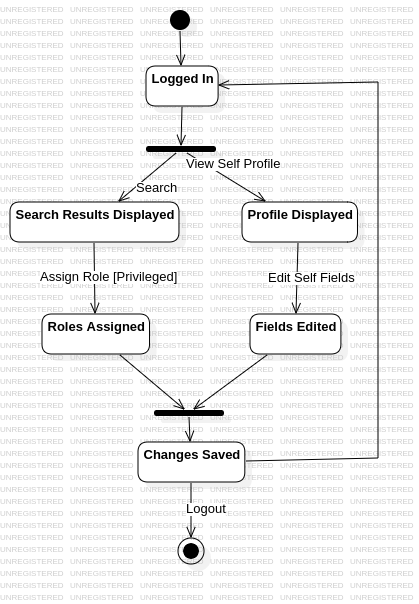
\includegraphics[height=4in]{state_diagrams/StateMachine1!UserProfile_1.png}
\end{center}

\subsection{News}
\begin{center}
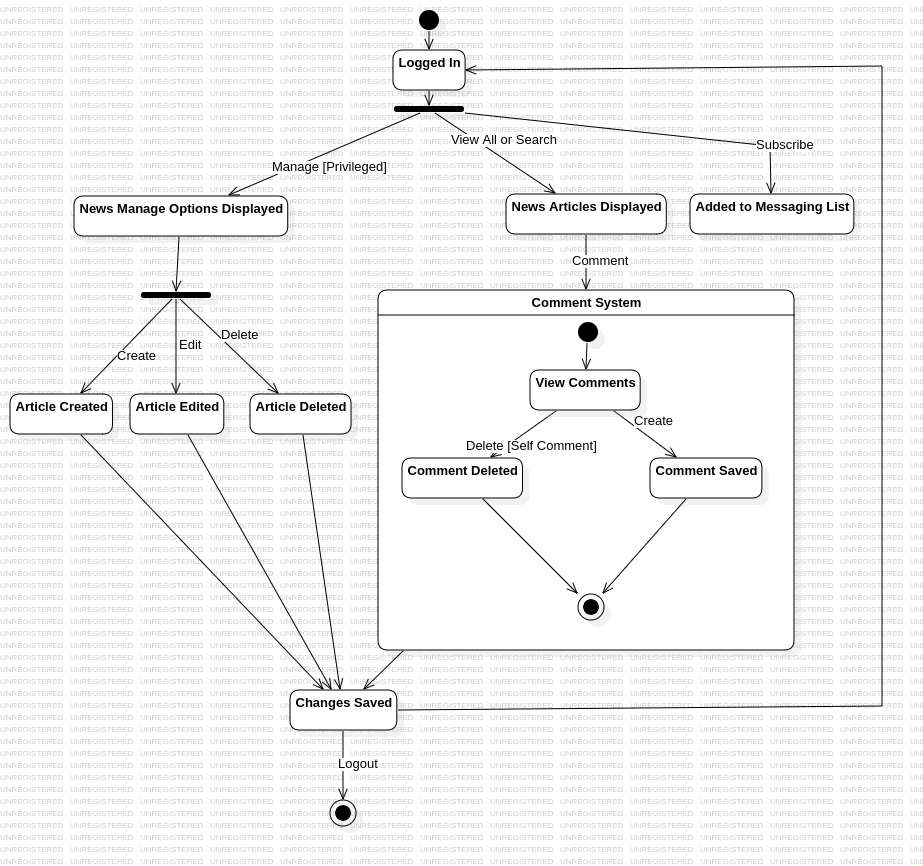
\includegraphics[height=4in]{state_diagrams/StateMachine2!News_2.png}
\end{center}

\subsection{Finance}
\begin{center}
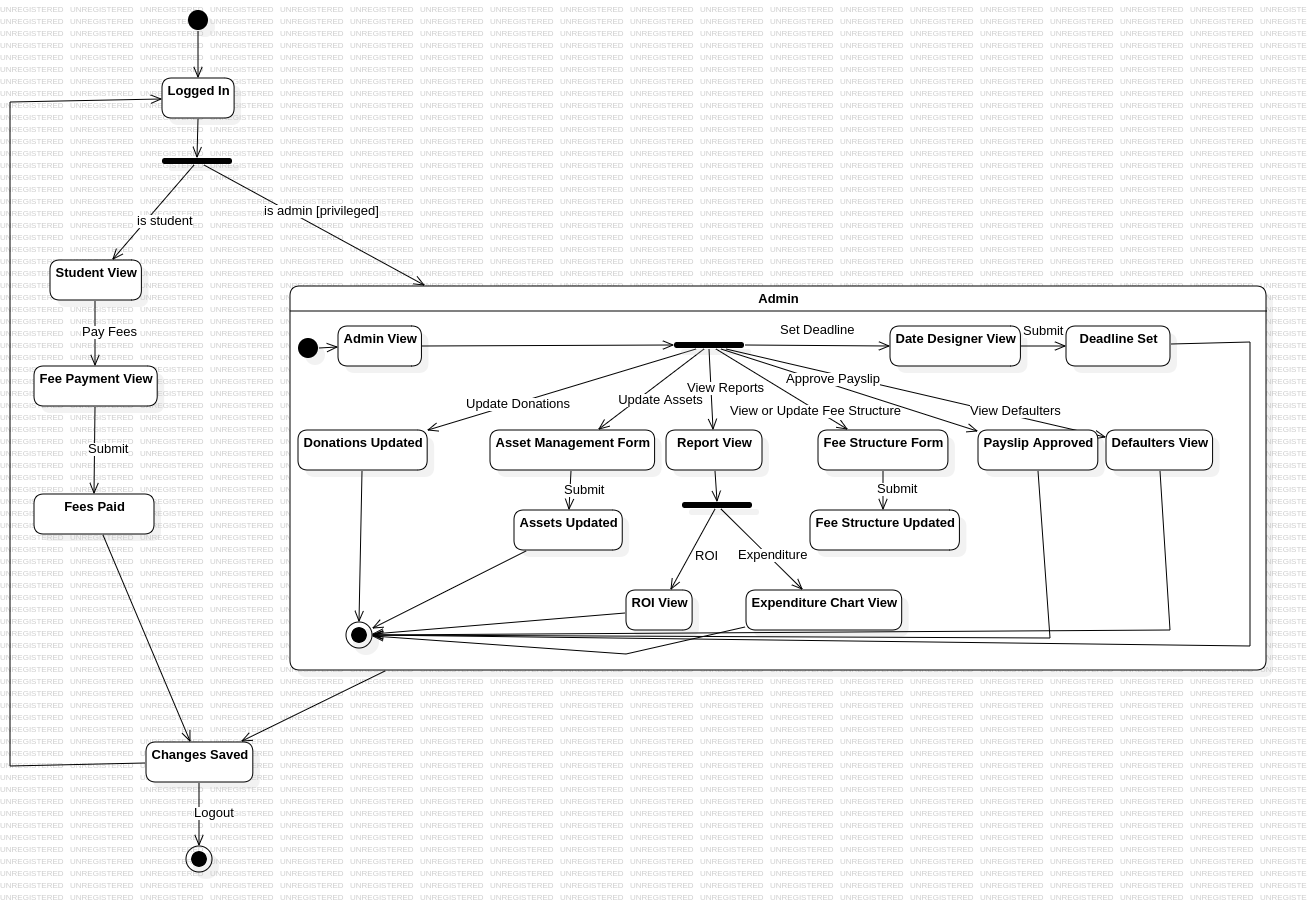
\includegraphics[height=4in]{state_diagrams/StateMachine4!Finance_3.png}
\end{center}

\subsection{Examination}
\begin{center}
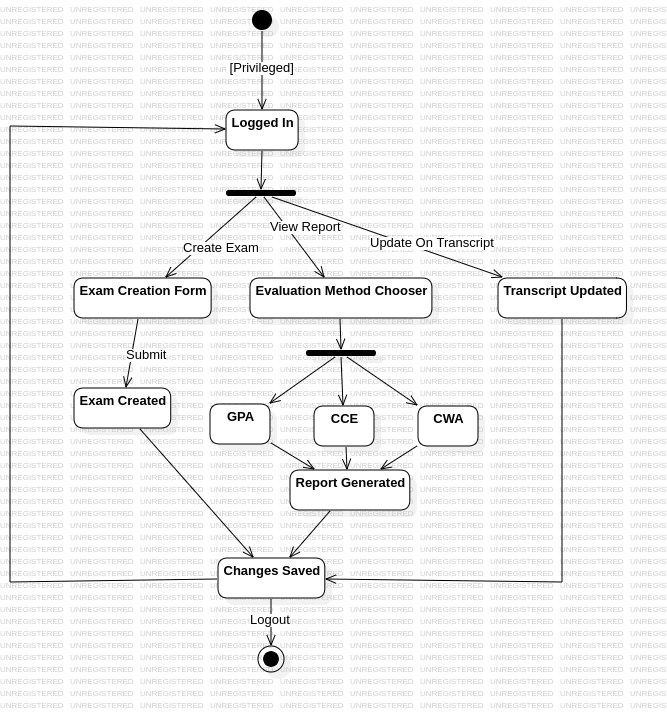
\includegraphics[height=4in]{state_diagrams/StateMachine5!Examination_4.png}
\end{center}

\subsection{Admission}
\begin{center}
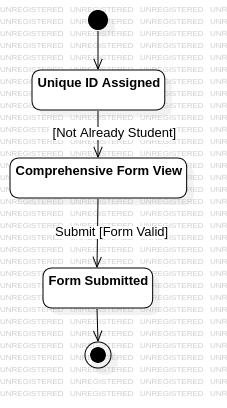
\includegraphics[height=4in]{state_diagrams/StateMachine6!Admission_5.png}
\end{center}



\section{Design Outline and Features}

\subsection{Low Coupling}
The design follows the principle of low coupling by separating concerns into distinct modules, such as User Management, Student Details, and Finance Management. Each module has a well-defined set of responsibilities and minimizes dependencies on other modules, allowing for easier maintenance and modification.

\subsection{High Cohesion}
The design promotes high cohesion by grouping related functionalities and data within the same module. For example, the Course and Batch Management module handles all aspects related to course definition, batch creation, student and faculty assignment, and class scheduling, ensuring that related operations are cohesively organized.

\subsection{Separation of Concerns}
The design separates different concerns into distinct modules, following the principle of separation of concerns. For instance, the User Management module handles user-related operations, while the Human Resource Management module focuses on employee-specific tasks, such as hiring, attendance tracking, and payroll processing.

\subsection{Modularity}
The design is structured as a modular system, with each module representing a distinct functional area. This modularity allows for better organization, maintainability, and scalability, as individual modules can be developed, tested, and updated independently.

\subsection{Information Hiding}
The design adheres to the principle of information hiding by encapsulating module-specific data and functionality within the respective modules. For example, the details of fee structure and invoicing are hidden within the Finance Management module, while the User Management module handles user-related information and operations.

\subsection{Extensibility}
The modular design promotes extensibility by allowing new functionalities or modules to be added without significantly impacting existing components. For instance, if a new requirement arises for managing hostels, a new module can be added to the system without disrupting other modules.

\subsection{Reusability}
The design encourages reusability by creating generic and reusable components or modules that can be shared across different parts of the system. For example, the Messaging System module can be reused for communication between different stakeholders, such as students, faculty, and administrators, reducing duplication of effort and promoting code reuse.

\section{Reflection on our Design}

These principles are integrated throughout the design to ensure a well-structured, maintainable, and scalable Institute Management System. The modular approach, clear separation of concerns, and adherence to principles like low coupling and high cohesion contribute to the overall quality and flexibility of the design.


\end{document}

